
\documentclass[border=10pt]{standalone}
\usepackage{pgfplots}
\pgfplotsset{compat=1.18}
\begin{document}
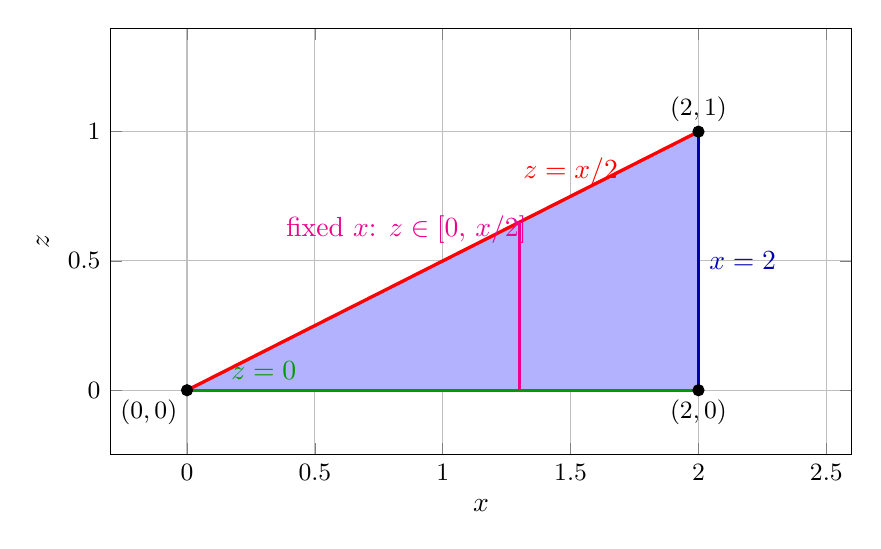
\begin{tikzpicture}
\begin{axis}[
    xlabel={$x$}, ylabel={$z$},
    xmin=-0.3, xmax=2.6, ymin=-0.25, ymax=1.4,
    width=11cm, height=7cm,
    grid=both,
    tick label style={font=\small},
]
\addplot[fill=blue!30,draw=none] coordinates {(0,0) (2,0) (2,1) (0,0)};
\addplot[green!60!black,very thick,domain=0:2,samples=2]{0} node[pos=0.15,above]{$z=0$};
\addplot[blue!70!black,very thick] coordinates {(2,0) (2,1)} node[pos=0.5,right]{$x=2$};
\addplot[red,very thick,domain=0:2,samples=2]{x/2} node[pos=0.75,above]{$z=x/2$};
% fixed-x indicator
\addplot[magenta,very thick] coordinates {(1.3,0) (1.3,0.65)};
\node[magenta,anchor=west] at (axis cs:0.35,0.62) {fixed $x$: $z\in[0,\,x/2]$};
\addplot[only marks,mark=*,mark size=2pt,black] coordinates {(0,0) (2,0) (2,1)};
\node[anchor=north east,font=\small] at (axis cs:0,0) {$(0,0)$};
\node[anchor=north,font=\small] at (axis cs:2,0) {$(2,0)$};
\node[anchor=south,font=\small] at (axis cs:2,1) {$(2,1)$};
\end{axis}
\end{tikzpicture}
\end{document}
